\documentclass[11pt]{article}
\setlength{\oddsidemargin}{0in}
\setlength{\evensidemargin}{0in}
\setlength{\textwidth}{6.5in}

\usepackage{fancyhdr}
\pagestyle{fancy}
\usepackage{amsmath,amsfonts,amssymb}
\usepackage{epsfig}
\usepackage{subfigure}
\usepackage{placeins}
\usepackage{amsmath}
\usepackage[usenames,dvipsnames,svgnames,table]{xcolor}
\usepackage{amssymb}
\usepackage{setspace}
\usepackage{graphicx} % Include figure files
\usepackage{times}
\usepackage{amsthm}
\usepackage{hyperref}
\usepackage{enumitem}
\hypersetup{bookmarks=true, unicode=false, pdftoolbar=true, pdfmenubar=true, pdffitwindow=false, pdfstartview={FitH}, pdfcreator={Daniel Larremore}, pdfproducer={Daniel Larremore}, pdfkeywords={} {} {}, pdfnewwindow=true, colorlinks=true, linkcolor=blue, citecolor=Green, filecolor=magenta, urlcolor=cyan,}
\usepackage[parfill]{parskip}

\graphicspath{{../Notes/PythonFigs/}{./}}

\newcommand{\e}{\mathrm{e}}
\renewcommand{\d}{\mathrm{d}}
\newcommand{\erf}{\mathop\mathrm{erf}}
\newcommand{\erfc}{\mathop\mathrm{erfc}}
\newcommand{\xmin}{\ensuremath{x_{\min}}}
\newcommand{\ntail}{\ensuremath{n_{\rm tail}}}

\newcommand{\Q}[1]{\footnote{\textcolor{blue}{#1}}}

\usepackage{tcolorbox}
\tcbuselibrary{breakable}

\begin{document}

\lhead{{\bf Mathematical \& Computational Modeling of Infectious Diseases \\ 
Homework 3}}
\rhead{{\bf D.B.\ Larremore\\2023}}
\renewcommand{\headrulewidth}{0.4pt}

{\bf Instructions:} 
\begin{itemize}[itemsep=-7pt]
	\item Please turn in a single PDF file. 
	\item Please share a link to your code, but do not attach the actual code. 
	\item Handwritten math (scanned and included in a PDF) is fine, but please watch out for 10MB+ file sizes!
\end{itemize}
\vspace{0.1in}\hrule

\begin{enumerate}
	\item The goal of this problem is to get you thinking about the constraints on population contact structure and contact matrices.
	
\begin{enumerate}[label=\alph*.]
	\item As one who is interested in modeling disease transmission on college campuses, you hire two teams to measure contact patterns on a nearby campus. The first team, led by Dan Pemic, tells you that there are $200$ faculty and $1800$ students, with a contact matrix of 
	$$C = \begin{pmatrix}
		3.1 & 43.5 \\
		4.7 & 25.0
	\end{pmatrix}$$
The second team, led by Flynn Uenza, tells you that there are $210$ faculty and $1750$ students, with a contact matrix of
	$$C = \begin{pmatrix}
		3.0 & 44.5 \\
		4.8 & 25.1
		\end{pmatrix}
	$$
Whom do you trust more, Dan Pemic or Flynn Uenza? Explain your reasoning in words and include any calculations used to arrive at your conclusions. 
\end{enumerate}

\begin{tcolorbox}
	\textbf{Solution}:\\
	First, let us clearly state our assumptions, the matrices $C$ are interpreted as the number of contacts seen by a single student or faculty in a given unit of time. Within category interactions are primarily due to social interaction and random chance. Further, assume that student-faculty and faculty-student interactions are due exclusively due to classroom interaction. In a classroom interaction, it is assumed that a single faculty interacts with every student and every student interacts with the single faculty. 
	
	With the above assumptions we consider the first scenario with $200$ faculty and $1800$ students. In a given unit of time, we should then expect the $200$ faculty to interact with $200*C_{1,2}=200*43.5=8700$ students and the $1800$ students to interact with $1800*C_{2, 1}=1800*4.7=8460$ faculty. Since these interactions are symmetric, they should be very close to the same to account for some empirical error. In this case there is a discrepancy of $240$ interactions.
	
	We repeat the same calculation for the second scenario and get a discrepancy of $945$ interactions. So at first inspection, Flynn Uenza's team does not immediately pass intuition since it does not account for the expected interactions, but given the populations are relatively small and measurement methods can introduce variance, neither team appears to have made a major mistake. Despite that, Dan Pemic's team seems like a safer option in absence of additional information.
\end{tcolorbox}

\clearpage
\item The goal of this problem is to explore the preferential depletion of susceptibles. 

Consider a population with four equal-sized groups, numbered $1, 2, 3, 4$. Suppose that the contact structure in the population is fully mixed (i.e. $c_{ij} = \bar{c}$ for all $i,j$), that $\gamma_i = 3$ for all $i$, and that $R_0=1.5$, under SIR dynamics. Finally, suppose that the susceptibility for group $1$ is $p_1=1$, the susceptibility for group $2$ is $p_2=2$, with $p_3 = 3$ and $p_4=4$. 

\begin{enumerate}[label=\alph*.]
	\item In terms of $\bar{c}$, $s_1$, $s_2$, $s_3$, and $s_4$ (and constants), what is the next-generation matrix for this system?
	
	\begin{tcolorbox}[breakable]
		\textbf{Solution}:\\
		We need to begin with the infection equations under SIR dynamics. We begin with the following set of equations
		\begin{align*}
			\dot{I_1}&=p_1 S_1 c_{11}\frac{I_1}{N_1} + p_1 S_1 c_{12}\frac{I_2}{N_2}+ p_1 S_1 c_{13}\frac{I_3}{N_3}+ p_1 S_1 c_{14}\frac{I_4}{N_4}-\gamma_1I_1\\
			&\vdots\\
			\dot{I_4}&=p_4 S_4 c_{41}\frac{I_1}{N_1} + p_4 S_4 c_{42}\frac{I_2}{N_2}+ p_4 S_4 c_{43}\frac{I_3}{N_3}+ p_1 S_4 c_{44}\frac{I_4}{N_4}-\gamma_4 I_4.
		\end{align*}
		This can be simplified by substituting in requisite values and noting that since all population sizes are equal, we have $\frac{I_j}{N_j}=i_j, \,\frac{s_j}{N_j}=s_j$, and our equations become
		\begin{align*}
		\dot{i_1}&=\bar{c}s_1(i_1 + i_2 +i_3+  i_4)-\gamma i_1\\
		&\vdots\\
		\dot{i_4}&=4\bar{c}s_4(i_1 + i_2+ i_3+  i_4)-\gamma i_4.
		\end{align*}
		Then, we write down our Jacobian as
		\begin{align*}
			J &= \begin{bmatrix}
			\bar{c}s_1-\gamma&\bar{c}s_1&\bar{c}s_1&\bar{c}s_1\\
			2\bar{c}s_1&2\bar{c}s_1-\gamma&2\bar{c}s_1&2\bar{c}s_1\\
			3\bar{c}s_1&3\bar{c}s_1&3\bar{c}s_1-\gamma&3\bar{c}s_1\\
			4\bar{c}s_1&4\bar{c}s_1&4\bar{c}s_1&4\bar{c}s_1-\gamma\\
			\end{bmatrix}\\
			&=
			\begin{bmatrix}
			\bar{c}s_1&\bar{c}s_1&\bar{c}s_1&\bar{c}s_1\\
			2\bar{c}s_1&2\bar{c}s_1&2\bar{c}s_1&2\bar{c}s_1\\
			3\bar{c}s_1&3\bar{c}s_1&3\bar{c}s_1&3\bar{c}s_1\\
			4\bar{c}s_1&4\bar{c}s_1&4\bar{c}s_1&4\bar{c}s_1\\
			\end{bmatrix}
			+
			\begin{bmatrix}
			-\gamma&0&0&0\\
			0&-\gamma&0&0\\
			0&0&-\gamma&0\\
			0&0&0&-\gamma
			\end{bmatrix}\\
			&=
			T + \Sigma.
		\end{align*}
		With this, we form $G=-T\Sigma^{-1}$ and
		\begin{equation*}
			G = \frac{1}{\gamma}T,
		\end{equation*}
		where $T$ is as above. This forms our next generation matrix.
	\end{tcolorbox}
	
	\item To ensure that $R_0=1.5$, what must $\bar{c}$ be equal to?
	
	\begin{tcolorbox}[breakable]
		\textbf{Solution}:\\
		For $R_0=1.5$, we need a specific $\bar{c}$. Keeping in mind $\gamma=3$, we look for the eigenvalues of $G$ when $s_j=1$ (that is, when the populations are all almost fully susceptible). Labeling this matrix $G_0$, we have
		\begin{equation*}
			G_0=\frac{\bar{c}}{3}\begin{bmatrix}
			1&1&1&1\\
			2&2&2&2\\
			3&3&3&3\\
			4&4&4&4
			\end{bmatrix}.
		\end{equation*}
		This system has only one non-zero eigenvalue at $\lambda = \frac{10 \bar{c}}{3}$. This is interpreted as $R_0$. Then for $R_0=1.5$, we simply require $\bar{c}=\frac{3}{10}1.5 = 0.45$.
	\end{tcolorbox}
	
	\item Using these parameters, code up a version of your model with initial conditions where $99.9\%$ of people in each group are susceptible, and the other $0.1\%$ are infected.\footnote{You'll have to modify your code to cope with the fact that there are now 4 groups!} Simulate an epidemic wave using an appropriate timestep $\Delta t$ and appropriate maximum simulation time to capture the wave. Create a plot of the four populations' $I$ compartments vs time, showing $i_1(t)$, $i_2(t)$, $i_3(t)$, and $i_4(t)$. Color these curves in a single hue, but with varying levels of light/dark or saturation, such that the boldest and darkest line is the most susceptible group, and the faintest and lightest line is the least susceptible group.
	
	\begin{tcolorbox}[breakable]
		\textbf{Solution}:\\
		Code used to generate the plot is on my github at https://github.com/WilliamMagrogan/InfectiousDiseaseModeling. 
	\end{tcolorbox}
	\begin{figure}
		\centering
		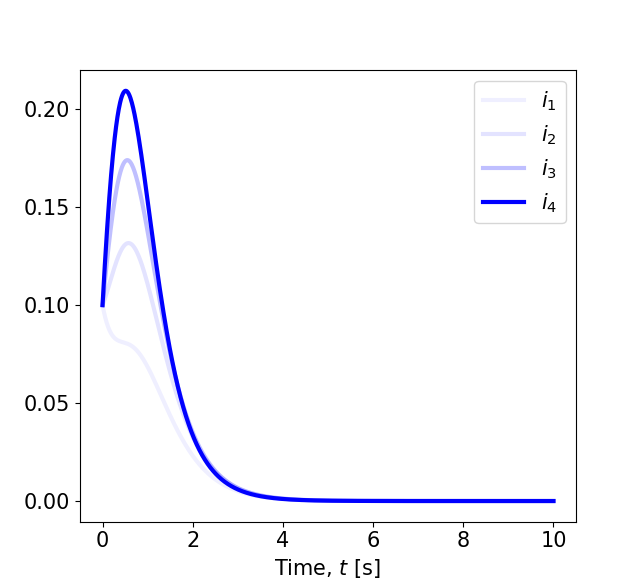
\includegraphics[scale=0.7]{problem2c.png}
	\end{figure}
	
	\item Define the average relative susceptibility among the susceptibles at any point in time $\bar{p}(t)$ as
	$$\bar{p}(t) = \frac{\displaystyle \sum_{i=1}^4 p_i\,s_i(t)}{\displaystyle \sum_{i=1}^4 s_i(t)}\ .$$
	Note that this is simply a weighted average of the susceptibilities of the susceptibles, by adding up the susceptibilities in the numerator and dividing by the number of susceptibles in the denominator. Over the same time window as your previous plot, create two addition figures: First, show $s_i(t)$ for each $i=1, 2, 3, 4$ using the same color scheme as before. Second, show $\bar{p}(t)$ in black. 
	
	\begin{tcolorbox}[breakable]
		\textbf{Solution}:\\
		Code to produce is again found on github.
	\end{tcolorbox}
	\begin{figure}
		\centering
		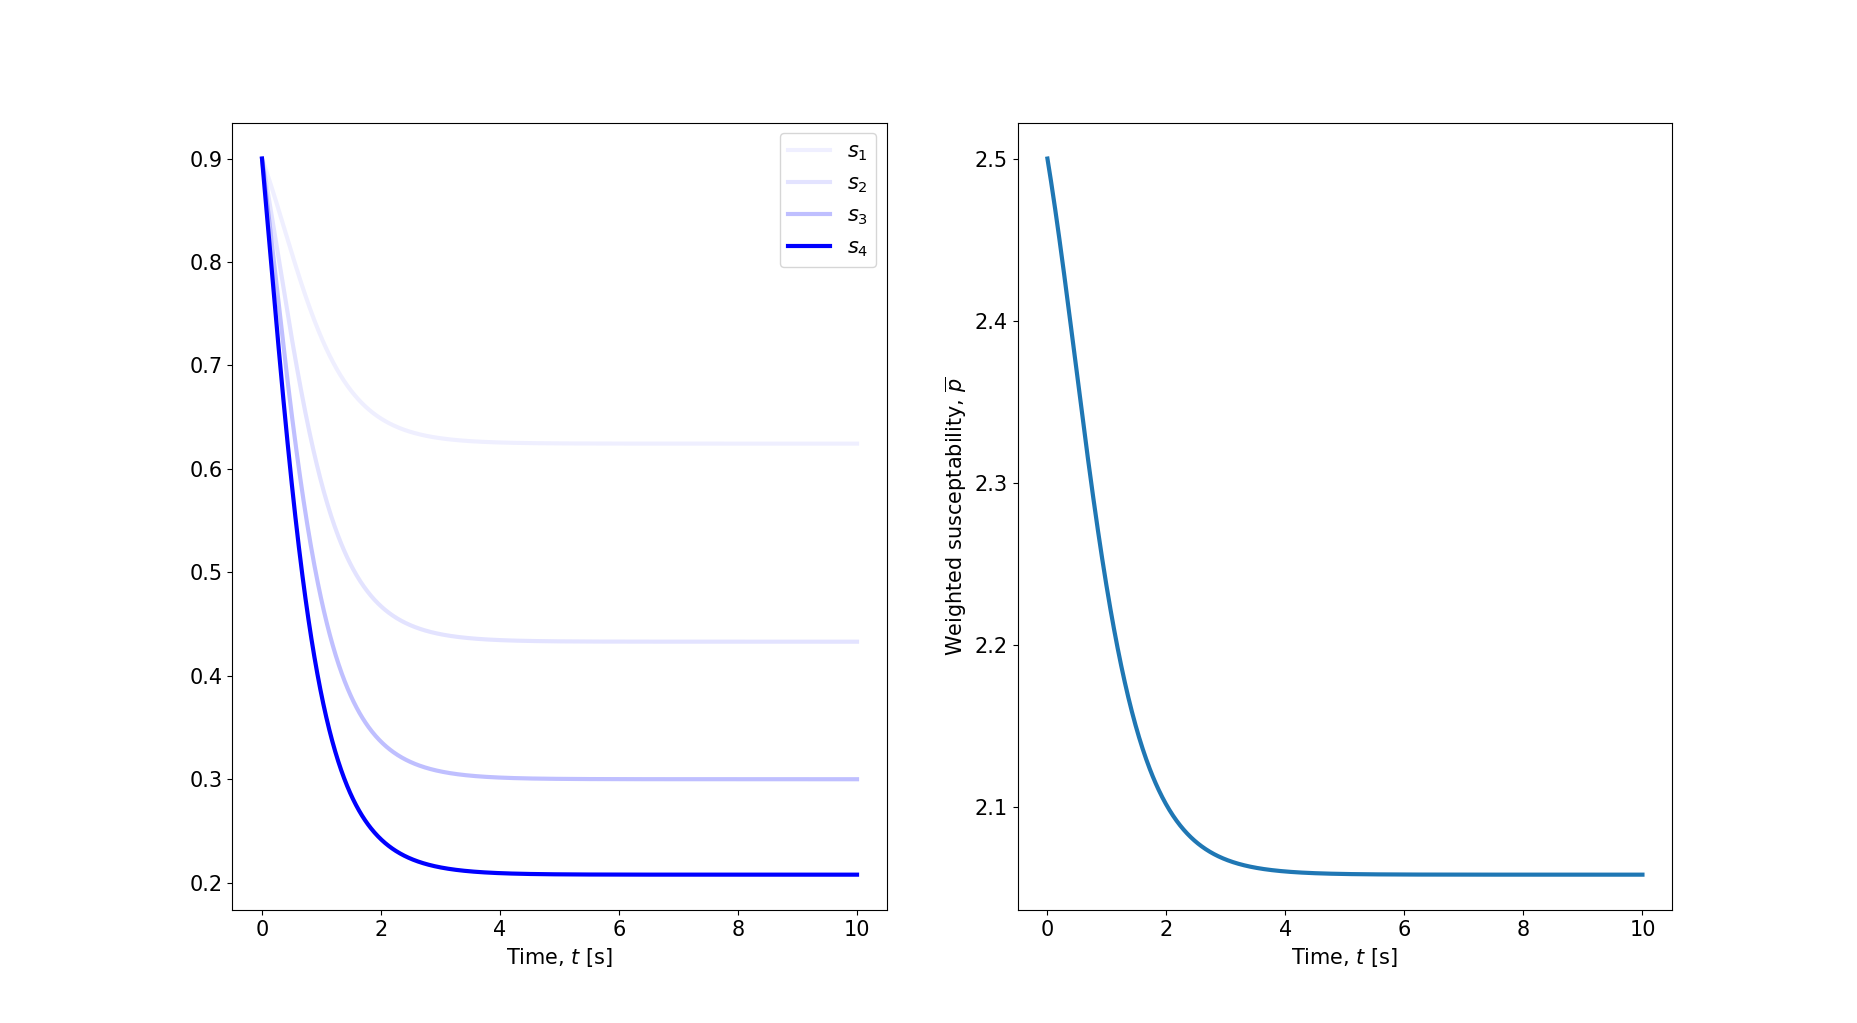
\includegraphics[scale=0.3]{problem2d.png}
	\end{figure}
	
	\item Comment on what you observe in the plots, and explain the reason for the patterns in words that a high school student could understand.
	
	\begin{tcolorbox}[breakable]
		\textbf{Solution}:\\
		We see that for the susceptible populations stabilize according to their risk, that is the most at risk one has the least uninfected members and the least at risk one has the most uninfected members. In the effective mean susceptibility plot, we note that at the beginning, it starts at $2.5$, the mean of $[1, 2, 3, 4]$ as expected since all the susceptible populations have concentration near $1$. As the epidemic progresses, and the pool or susceptible people is composed of more low susceptibility people and fewer high susceptibility people, the effective susceptibility decreases until saturation is reached at a weighted mean of their saturated susceptibilities. 
	\end{tcolorbox}
	
	\item[Extra Credit] Reflect on these plots in the context of the COVID-19 pandemic. What lessons are there to be drawn from the relationship between an epidemic wave and different groups with different susceptibilities?
	
	\begin{tcolorbox}[breakable]
		\textbf{Solution}:\\
		One of the main commentaries that was discussed during the COVID-19 pandemic was regarding the role of essential workers, those who were required to continue working and likely interacting with individuals on a regular basis. The immuno-compromised were another frequently discussed group. Both of these, for different reasons, can be considered their own groups for purposes of modeling. The immuno-compromised because of their higher susceptibility on a per-contact basis, and the essential workers due to their inherent higher contact rate. Understanding the needs and unique behaviors and susceptibilities of these respective groups is critical to good modeling and robust public policy.
	\end{tcolorbox}
\end{enumerate}
\clearpage

\item The goal of this problem is to explore branching processes, and how superspreading can, perhaps surprisingly, increase the likelihood that an outbreak never grows to a large size.

This problem introduces the {\bf negative binomial} (NB) distribution. The distribution can be parameterized a few different ways, but for our purposes, it will be convenient to specify a mean and a dispersion. In the context of transmission chains and branching processes, drawing the number of secondary infections from a negative binomial requires that the mean be $R_0$. However, the dispersion parameter allows us flexibility, and importantly, allows us to model superspreading. 

When $k \to \infty$, the negative binomial distribution converges to a Poisson distribution. When $k = 1$, the negative binomial is equivalent to a geometric distribution. A key difference between these is that the mode of a Poisson---its most common value---is around its mean, while the mode of a Geometric is zero. In the context of branching processes, this means that a high $k$ will lead to more similar numbers of secondary infections for each primary infection. In contrast, a low $k$ will lead to many instances where there are just a few (or zero) secondary infections, and rare instances with a large number of secondary infections. When $k$ is low, we often talk about ``superspreaders,'' people whose infections lead to an exceptionally larger number of secondary infections. 

Note: You can find Python code to draw from a negative binomial with the $R_0$ and $k$ parameterization provided on the next page. For those writing in other languages, be careful to use the correct parameterization (mean and dispersion).

\begin{enumerate}[label=\alph*.]
	\item Write code for a branching process that, starting from a single infection, draws $G$ generations, with each infection creating $NB(R_0,k)$ additional infections. Use your code to estimate $q$ the probability\footnote{See class notes.} that an epidemic dies in finite time, for $R_0=3$ and $k=0.1, 0.5, 1.0, 5.0,$ and $10.0$.\footnote{Hint: When we estimate a probability from a stochastic process like this, a convenient way to do this is Monte Carlo: simulate, say, $100,000$ branching processes and take note of how many cease before growing large.} Provided your answers in a table, out to 3 decimal places.
	
	\begin{tcolorbox}[breakable]
		\textbf{Solution}:\\
		Here we take, for practicality sake, the assumption that if a branching process does not die out in fewer than $5$ generations, it continues forever. Then, running $10,000$ simulations at each parameter set, the probability that the outbreak does not die out, $q$, is estimated by 
		\begin{equation*}
			q \sim 1 - \frac{\text{count of finite time die-outs}}{\text{simulation runs}}.
		\end{equation*}
		\begin{center}
			\begin{tabular}{|c | c|}
				$k$ & Estimate of $q$\\
				0.1&0.167\\
				0.5&0.548\\
				1.0&0.670\\
				5.0&0.878\\
			\end{tabular}
		\end{center}
		
	\end{tcolorbox}
	
	\item How does $k$ affect $q$? Explain what this means in terms of the relationship between $p$ (i.e., $1-q$) and superspreading. 
	
	\begin{tcolorbox}[breakable]
		\textbf{Solution}:\\
		There is a clear positive relationship between $k$ and the estimate of $q$, and subsequently a negative relationship between $k$ and $p$. Intuitively, this tells us that as $k\rightarrow \infty$, and the negative binomial approaches a Poisson distribution, the probability of a finite time die-out drops precipitously to $0$.\\
		This can be thought of in terms of superspreading. In a superspreading scenario, a small handful of individuals are responsible for the majority of secondary contacts. Lower $k$ means the superspreaders donimate the secondary infections even more. Then, one can thing of an infinite outbreak occuring if you hit one of the superspreaders. Now, there is a competing effect: will an infection reach a superspreader and become massive or die out before it gets there. So, for very low $k$, the number of superspreaders is low, and the number of connections to reach them will be increasingly low. So, smaller $k$ means a mass outbreak is less likely to happen, but also, that it will likely be even bigger.
		
	\end{tcolorbox}
	
	\item [Extra Credit] How large do finite outbreaks get before they die out? For the parameters above, and for only the {\it finite} outbreaks, plot a histogram of $100,000$ finite outbreaks for your choice or choices of $k$, and $R_0=3$. What do you observe? 
	
	\begin{tcolorbox}[breakable]
		\textbf{Solution}:\\
		Here we take $k=0.1$. We have plotted, the data as a histogram on a logscale. Note, due to the restriction of no outbreaks greater than $5$ generations, there are likely outbreaks of a greater size than shown. \\
		From the data, we can see that the size of the largest outbreaks seen is just shy of $10^2=100$. Further, the data does not appear to be linear in log-space, which indicates it is probably not a simple power law relationship between outbreak size and its probability of happening.
	\end{tcolorbox}
	\begin{figure}
		\centering
		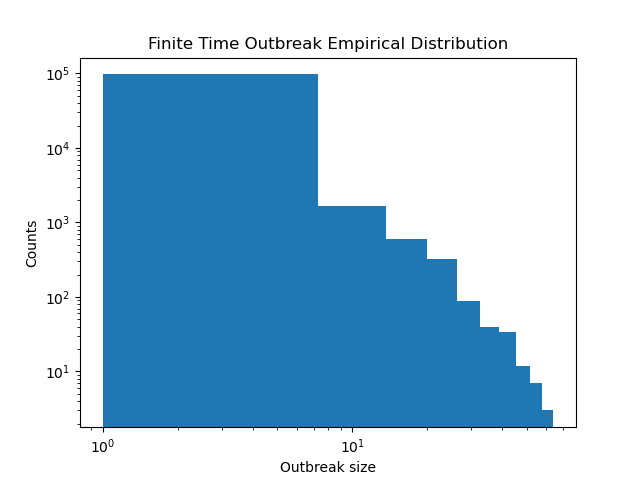
\includegraphics[scale=0.7]{problem3ec.png}
	\end{figure}

	
\end{enumerate}

\clearpage
Here is some Python code to draw from $NB(R_0, k)$:
\begin{verbatim}
from scipy.stats import nbinom

k = 10000 # Dispersion Parameter k
R0 = 3 # Mean R0

mean = R0
variance = mean + (mean**2)/k
p = mean/variance
n = mean**2 / (variance - mean) 

draw = nbinom.rvs(n=n,p=p)
draws = nbinom.rvs(n=n,p=p,size=10)
\end{verbatim}



\end{enumerate}

\end{document}